\begin{quote}
That was exhausting.
\end{quote}

The old blog post?

\begin{quote}
Yes. Exhausting in the sense that you have to hold three versions of yourself in your head at once. You have to hold in your mind the version of you who, in 1998, had such a large panic attack that he ran away from home. You have to hold in your mind the version of you who, in 2015, was struggling through the early stages of transition, who was finally getting into the meat of things with therapy. And you have to hold me in your mind.
\end{quote}

You have to remember that I'm powered by a small cantaloupe. Holding all three of those in my head at once would be a bit much.

\begin{quote}
One of us was getting squeezed out.
\end{quote}

Did you feel neglected?

\begin{quote}
That's nostalgia: neglect of the present in favor of the past.
\end{quote}

I suppose it is. I'll refrain from diving into a blog post like that again.

\begin{quote}
You can, just mind your boundaries.
\end{quote}

I will.

\begin{quote}
Tell me about running away.
\end{quote}

Again?

\begin{quote}
You-who-live-in-2019, tell me about running away.
\end{quote}

One of us mentioned before that it was the moment at which I started to assert ownership over myself.

\begin{quote}
We both did.
\end{quote}

I suppose I stand by that, then. Stand by the idea that that was conception to the birth that came in high school.

But it needs some qualifications.

\begin{quote}
Qualify away.
\end{quote}

One qualification that it needs is that, at the moment, just as with so many other forms of conception, it was borne of some baser part of me. It was not some conscious thing. It was not this clean and well-thought-out experience, sleek by design.

It was a release of terror into action. I was blacking out from fear. I was so full of adrenaline that living my life as a vagrant was more acceptable to me than waiting for my dad to come home. It was an act that happened. Not something I did.

\begin{quote}
Some folks try to conceive.
\end{quote}

Fair.

Some folks try and plan out their memoirs.

\begin{quote}
Fair.
\end{quote}

Another qualification that needs to be made is that, while I'm willing to accept this was about the time I started to assert ownership over myself, I don't think it happened while running away. Not that night.

\begin{quote}
When did it happen?
\end{quote}

It happened that morning when I sat atop the rocks of Rock Park. I sat atop the rocks and watched kids walking along the cul-de-sac toward Eisenhower, my old Elementary school.

I watched them walking and thought about how much bigger their backpacks looked than mine did when I was in school.

I watched them and I thought about how big my backpack might get in high school, and realized that I wouldn't find out.

I watched them and I thought about going to knock on the door at my mom's house. It was five blocks away.

\begin{quote}
And then you chose not to.
\end{quote}

Yes.

\begin{quote}
Dig deeper.
\end{quote}

\begin{figure}
\centering
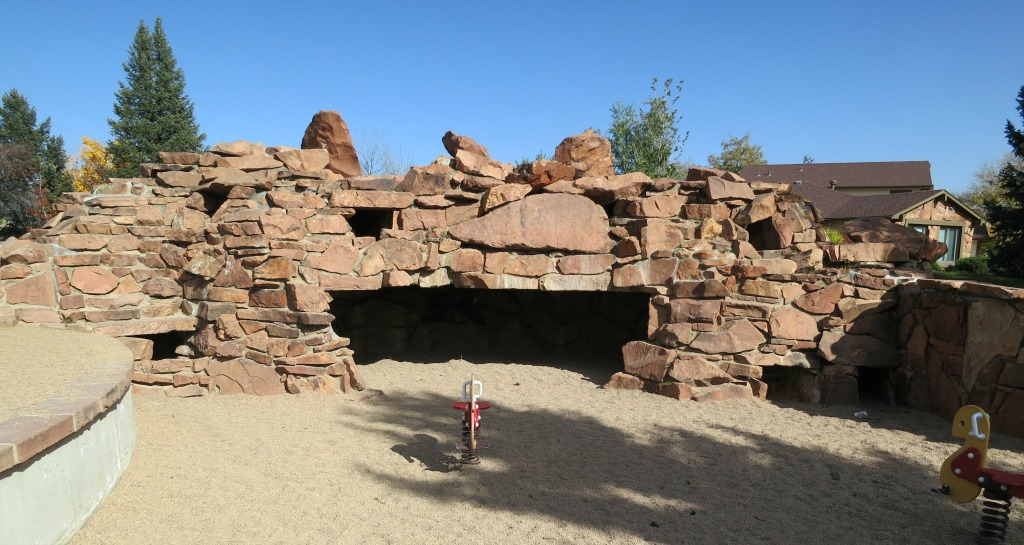
\includegraphics{/rock-park.jpg}
\caption{Rock park}
\end{figure}
